\documentclass[aspectratio=43]{beamer}

\mode<presentation>
{
  \usetheme{Spil}
  \setbeamercovered{invisible}
}

\usepackage[english]{babel}
\usepackage[latin1]{inputenc}

\usepackage{times}
\usepackage[T1]{fontenc}

% Anchoring images
%\usepackage[absolute, overlay]{textpos}

\title[]{\alert{Spilgames Storage Platform}}

\author[]{Enrique Paz}
%\author{\texorpdfstring{Author\newline\url{email@email.com}}{Author}}

\institute[] % (optional, but mostly needed)
{Senior Backend Developer}

\date[]{21/03/2013}

\AtBeginSection[]{
    \begin{frame}
        \begin{center}
            \huge{\insertsectionhead}
        \end{center}
    \end{frame}
}

\begin{document}

\begin{frame}
    \titlepage
\end{frame}

\section{Introduction}
\subsection{Spilgames \& Me}

\begin{frame}{About Me}
    \begin{columns}
        \begin{column}[c]{0.05\textwidth}
        \end{column}
        \begin{column}[c]{0.2\textwidth}
            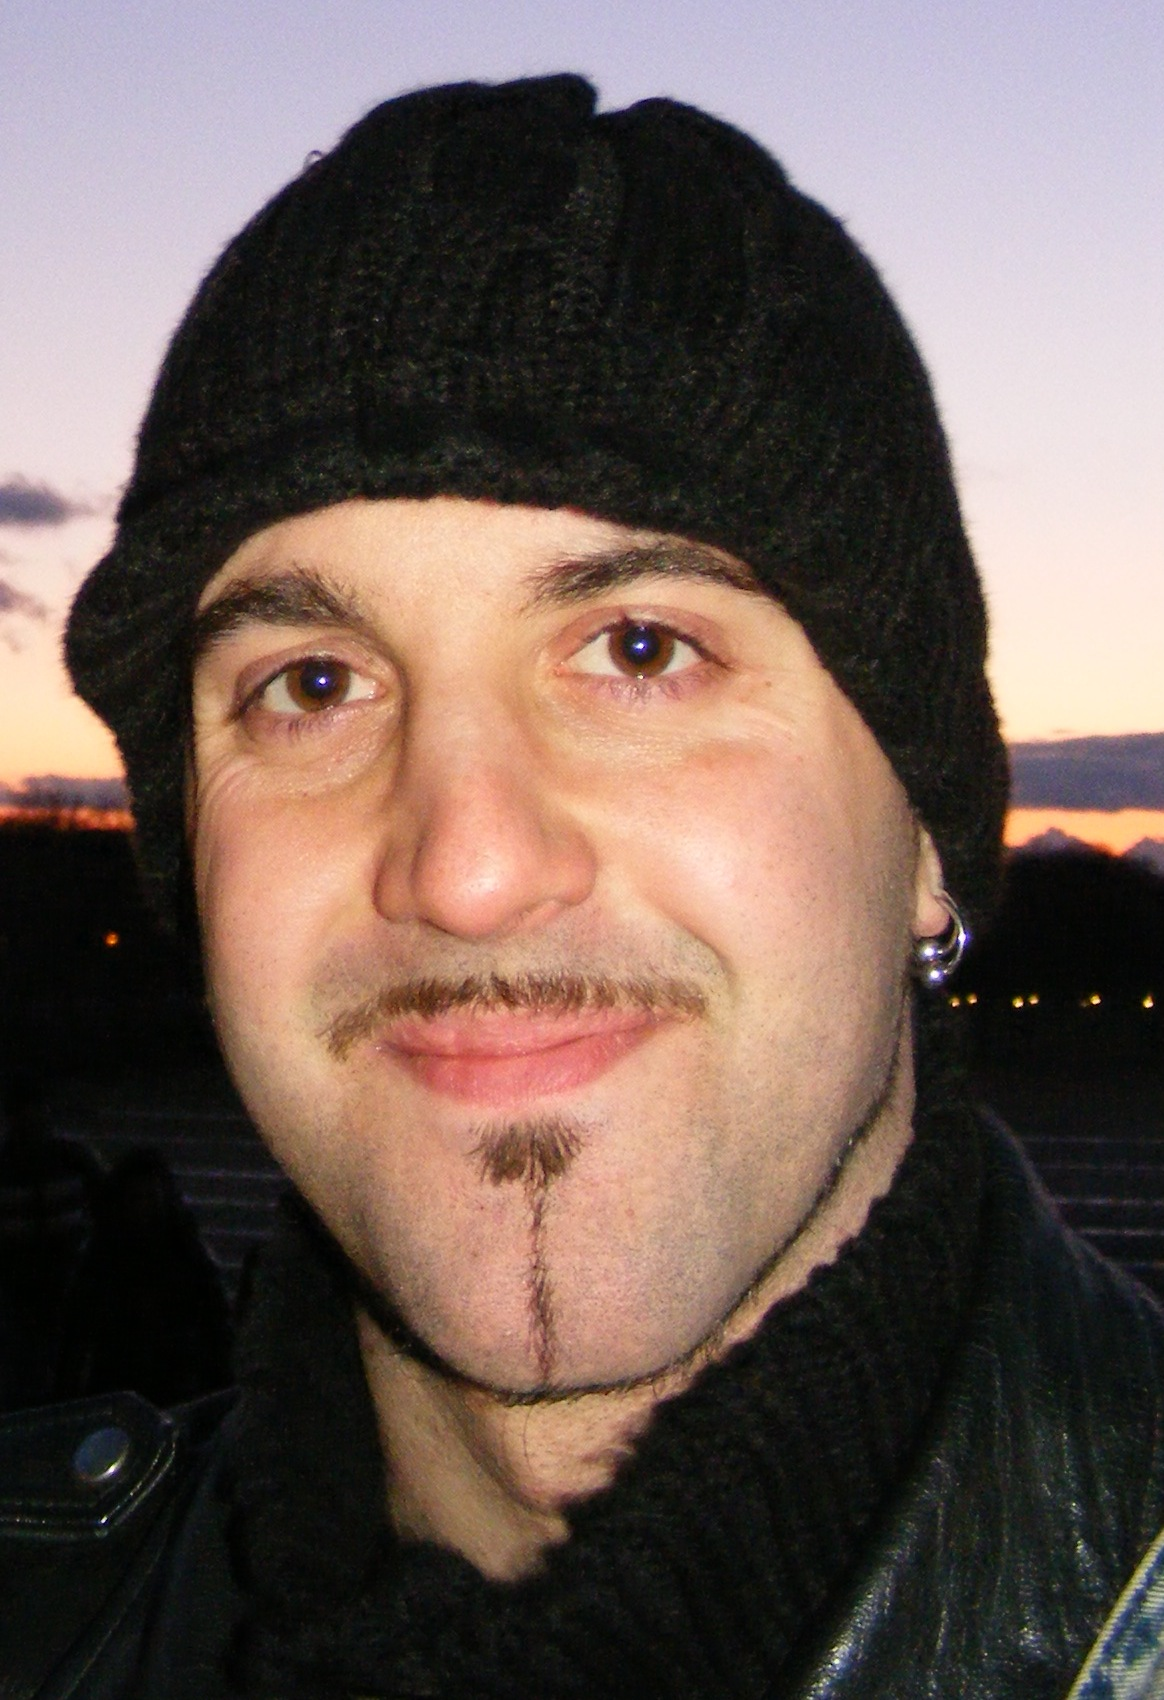
\includegraphics[width=\textwidth]{images/me.png}
        \end{column}
        \begin{column}[c]{0.05\textwidth}
        \end{column}
        \begin{column}[c]{0.7\textwidth}
            \begin{itemize}
                \item Passionate Erlang developer
                \item Testing enthusiast
                \item Love beautiful code!
            \end{itemize}
        \end{column}
    \end{columns}
\end{frame}

\begin{frame}{Spilgames}
    \begin{itemize}
       \item Gaming Platform
       \item Serving data to 190+ countries world-wide
       \item 200+ million unique users per month
       \item Multiple Platforms: Desktop, Mobile Native \& Web
       \item 300+ employees
       \item Offices in The Netherlands \& China
       \item Revenue: Advertising \& EUM
    \end{itemize}
\end{frame}

\begin{frame}{Gaming Portals}
    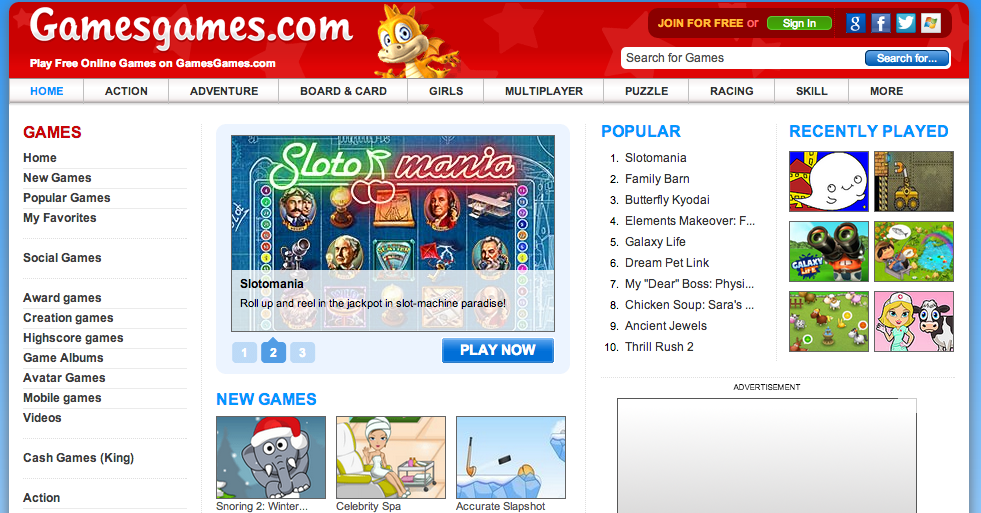
\includegraphics[width=\textwidth]{images/gamesgames.png}
\end{frame}

\begin{frame}{Gaming Portals}
    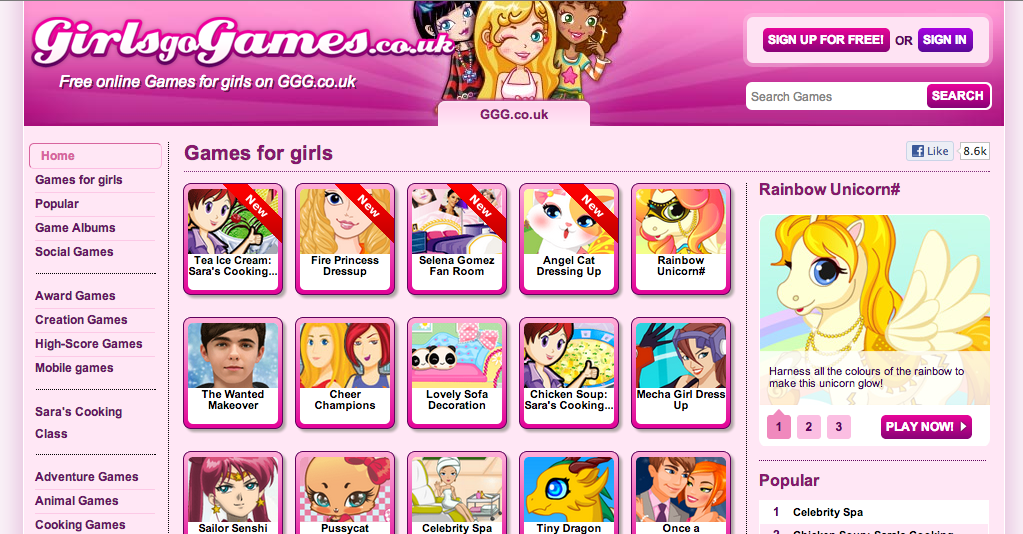
\includegraphics[width=\textwidth]{images/ggg.png}
\end{frame}

\begin{frame}{Games}
    \begin{columns}
        \begin{column}[c]{0.5\textwidth}
            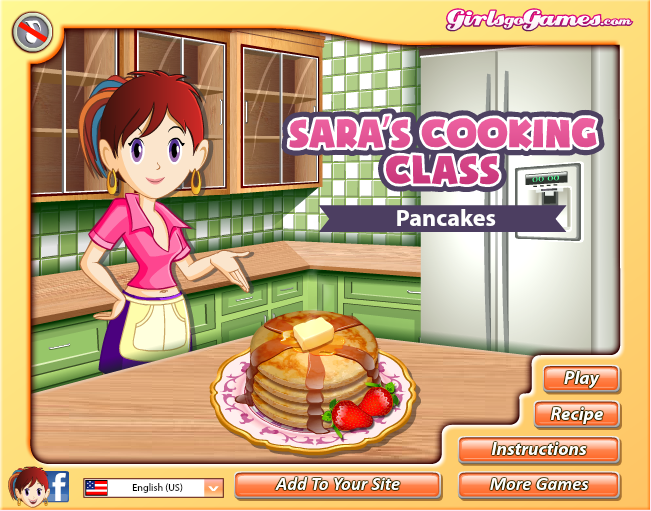
\includegraphics[width=\textwidth]{images/sarah.png}
        \end{column}
        \begin{column}[c]{0.5\textwidth}
            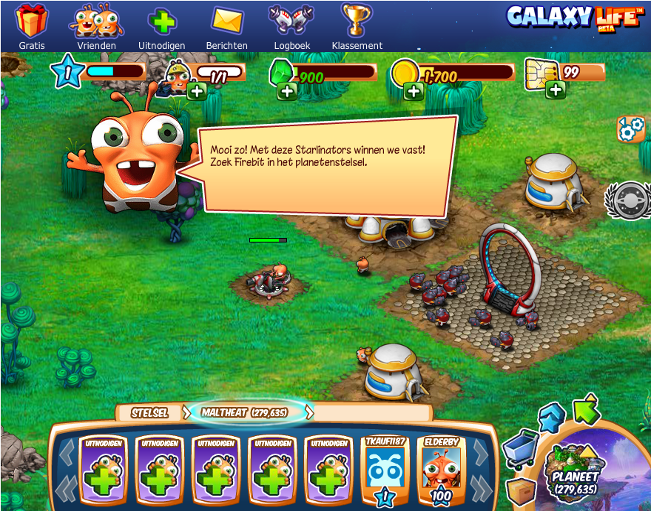
\includegraphics[width=\textwidth]{images/galaxylife.png}
        \end{column}
    \end{columns}
\end{frame}

\section{Another Storage}

{
\usebackgroundtemplate{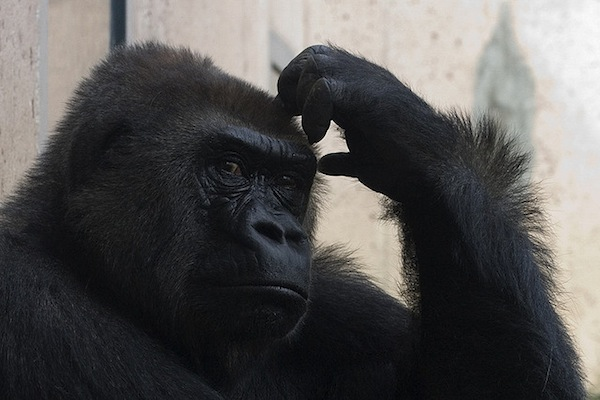
\includegraphics[height=\paperheight]{images/anotherstorage.png}}
\begin{frame}{Another Storage}
\end{frame}
}

\subsection{Motivation}

\begin{frame}{LAMP Stack \& MySql}
    \begin{columns}
        \begin{column}[c]{0.5\textwidth}
            \begin{itemize}
                \item Not all developers are DB experts
                \item Difficult to shard the databases
                \item Storage model all over the place
                \item Security
                \item Performance
                \item Caching
                \item \dots
            \end{itemize}
        \end{column}
        \begin{column}[c]{0.5\textwidth}
            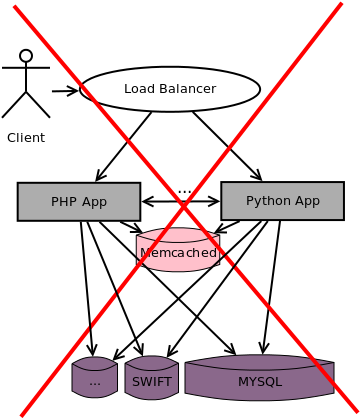
\includegraphics[width=0.9\textwidth]{images/oldstorageusage.png}
        \end{column}
    \end{columns}
\end{frame}

\begin{frame}{Our Ambition}
    \begin{columns}
        \begin{column}[c]{0.5\textwidth}
            \begin{itemize}
                \item Transparent sharding layer
                \item Sharding on data ownership
                \item High availability
                \item Centralized caching layer
                \item Storage engine agnostic
                \item One strict data model
                \item Transparent storage changes
                \item Scaling geographically
            \end{itemize}
        \end{column}
        \begin{column}[c]{0.5\textwidth}
            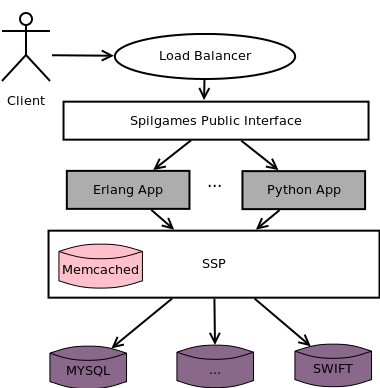
\includegraphics[width=\textwidth]{images/newstorageusage.png}
        \end{column}
    \end{columns}
\end{frame}

\section{System Properties}

\subsection{Overview}

\begin{frame}{Mindset}
    \begin{itemize}
        \item Be always available
        \item Avoid global locks
        \item Accept change as the only constant
        \item Embrace inconsistencies
            \begin{itemize}
                \item Hardware breaks down (power failures)
                \item Version mismatches (upgrading system not atomic)
                \item State mismatches (adding new machines)
            \end{itemize}
    \end{itemize}
\end{frame}

\begin{frame}{A Key-Value Store With Schema}
    \begin{itemize}
        \item \textbf{Buckets}
            \begin{itemize}
                \item Largely generated OTP applications
                \item Offer a CRUD-like interface (with filters)
            \end{itemize}
        \item \textbf{GID}s (64 bits) identify the data owner
            \begin{itemize}
                \item user
                \item game
            \end{itemize}
        \item Buckets can use different \textbf{storage engines}
            \begin{itemize}
                \item Several MySql tables in different databases
                \item Just a binary storage (SWIFT)
                \item \dots
            \end{itemize}
        \item Data for a bucket/GID is cached
        \item Requests can be atomic per bucket/GID
    \end{itemize}
\end{frame}

\begin{frame}{Optimistic Operations}
    \begin{itemize}
        \item Speed > Consistency
        \item Losing some updates in case of crash is affordable
        \item Act first on cache and then on disk
        \item No warranties of eventual consistency upon crashes
            \begin{itemize}
                \item i.e. Activity feeds
                \item i.e. Popular games list
            \end{itemize}
    \end{itemize}
\end{frame}

\begin{frame}{Pessimistic Operations}
    \begin{itemize}
        \item Consistency is key and confirmation is required
        \item Dealing with critical data
        \item Persist data and, upon success, update cache
            \begin{itemize}
                \item i.e. Payments
                \item i.e. Personal information
            \end{itemize}
    \end{itemize}
\end{frame}

\subsection{Internals}
{
\usebackgroundtemplate{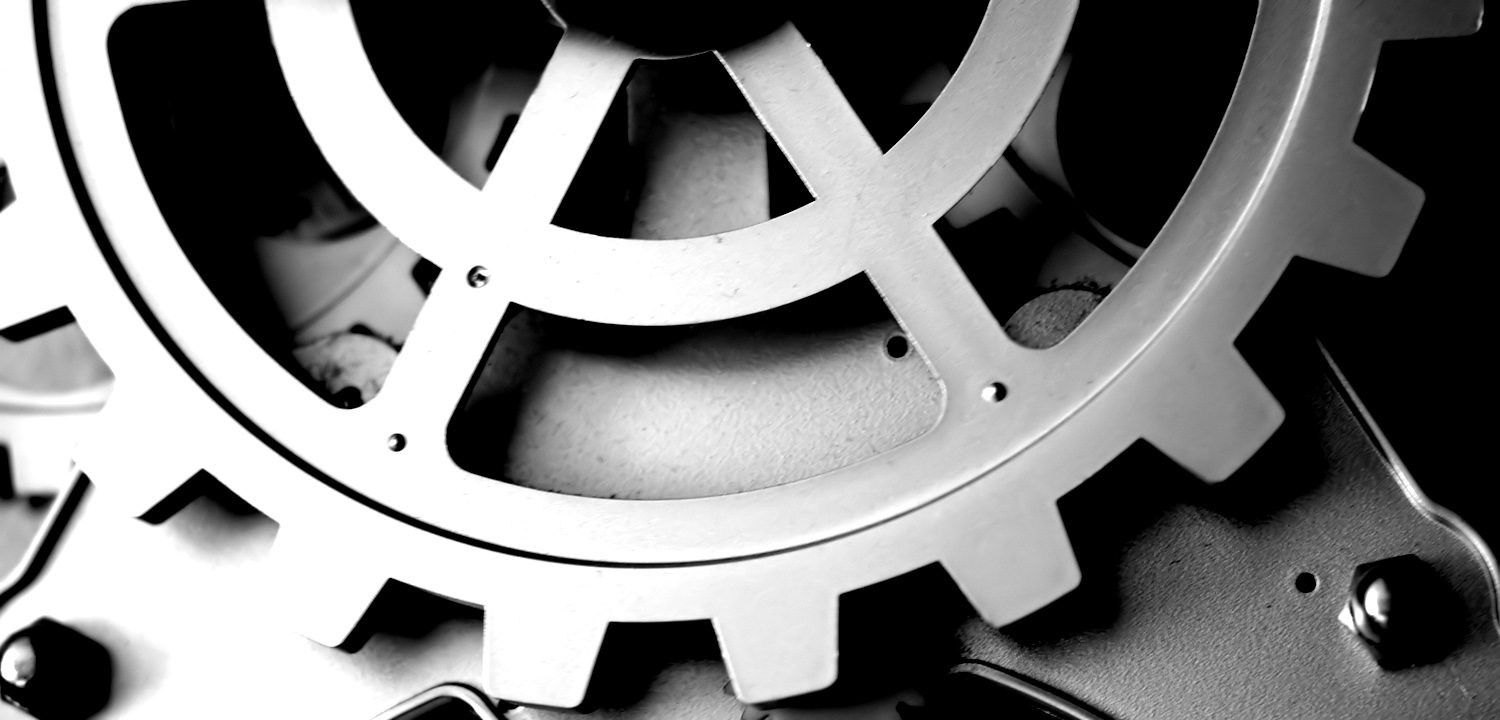
\includegraphics[height=\paperheight]{images/howitworks.png}}
\begin{frame}{How does it work?}
\end{frame}
}

\begin{frame}{System Components}
    \begin{columns}
        \begin{column}[c]{0.5\textwidth}
            \begin{itemize}
                \item \textbf{lookup} application in all nodes.\\
                      Uses a \textbf{hashing ring} (mnesia):
                            \begin{itemize}
                                \item replicated in all nodes
                                \item ram\_copies
                                \item dirty reads
                                \item transactional writes
                            \end{itemize}
                \item \textbf{Buckets} have Pipeline Factories
                \item Buckets register \textbf{PF}s in lookup
            \end{itemize}
        \end{column}
        \begin{column}[c]{0.5\textwidth}
            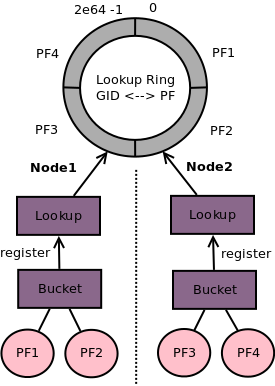
\includegraphics[width=0.9\textwidth]{images/components.png}
        \end{column}
    \end{columns}
\end{frame}

\begin{frame}{Tracing Pessimistic Operations}
    \begin{columns}
        \begin{column}[c]{0.5\textwidth}
            \begin{enumerate}
                \item Bucket/GID request in a node
                \item Local lookup to find a PF
                \item PF receives request
                \item PF builds job
                \item PF ensures Pipeline for GID
                \item PF queues operation in Pipeline
            \end{enumerate}
        \end{column}
        \begin{column}[c]{0.5\textwidth}
            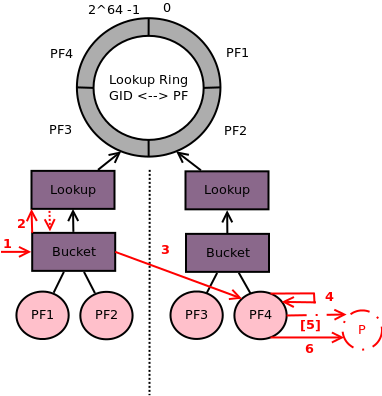
\includegraphics[width=\textwidth]{images/tracingpessimistic.png}
        \end{column}
    \end{columns}
\end{frame}

\begin{frame}{Wait a minute\dots}
    \begin{columns}
        \begin{column}[c]{0.5\textwidth}
            \begin{itemize}
                \item ``Why do we need pipelines?''
                \item ``Sequential == Bottleneck !!!''
                \item ``Don't you guys know Erlang is about \textbf{parallelizing} work?''
            \end{itemize}
        \end{column}
        \begin{column}[c]{0.5\textwidth}
            
\includegraphics[width=0.8\textwidth]{images/slow.png}
        \end{column}
    \end{columns}
\end{frame}

\begin{frame}{About Pipelines}
    \begin{itemize}
        \item \textbf{CONS}
            \begin{itemize}
                \item Sequential (read) access for hotspots\\
                    i.e. Popular games
                \item Optimization: read from SSP cache in PF
            \end{itemize}
        \pause
        \item \textbf{PROS}
            \begin{itemize}
                \item No need for storage engines to support global locks
                \item A bucket can combine several engines
            \end{itemize}
        \pause
        \item Requests to most GIDs (users) are evenly distributed
    \end{itemize}
\end{frame}

\subsection{Versions \& Shards}

\begin{frame}{Schema Versions}
    \begin{itemize}
        \item Schema Versions determine allowed operations and storage(s)
        \item Client is not aware of them
        \item Max 2 schema versions of a bucket at the time
        \item Schema version can be changed at bucket/GID level
    \end{itemize}
\end{frame}

\begin{frame}{Shards}
    \begin{itemize}
        \item Useful for partitioning big blocks of data
        \item Shard points to the physical location of the data
        \item Sharding rules are bucket specific. Default is GID \% Shards
        \item bucket/GID combinations can be migrated between shards
    \end{itemize}
\end{frame}

\begin{frame}{Working With Versions \& Shards}
    \begin{columns}
        \begin{column}[c]{0.5\textwidth}
            \begin{enumerate}
                \item \emph{insert(Bucket, Gid, Value)}
                \item \emph{insert(Gid, Value)}
                \item \emph{get\_vs(Bucket, Gid)}
                \item \emph{\{v2, Shard1\}}
                \item \emph{build\_job(insert, Gid, Shard1)}
                \item \emph{\{ok, InsertJob\}}
                \item \emph{\{ok, InsertJob\}}
                \item \emph{queue(InsertJob)}
            \end{enumerate}
        \end{column}
        \begin{column}[c]{0.5\textwidth}
            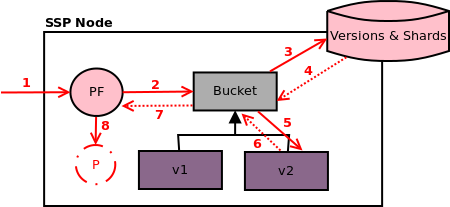
\includegraphics[width=\textwidth]{images/versionsandshards.png}
        \end{column}
    \end{columns}
\end{frame}

\begin{frame}{One API To Rule Them All}
    \begin{itemize}
        \item ``Don't care where it is, just want my data!!!''
        \pause
        \item \href{http://piqi.org}{PIQI} helps with the API
        \begin{columns}
            \begin{column}[c]{0.3\textwidth}
                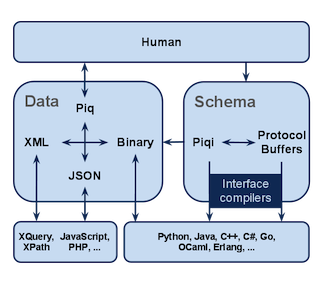
\includegraphics[width=\textwidth]{images/piqi.png}
            \end{column}
            \begin{column}[c]{0.6\textwidth}
                \begin{itemize}
                    \item Erlang client + Protocol Buffers
                    \item HTTP + JSON
                    \item HTTP + Protocol Buffers
                \end{itemize}
            \end{column}
        \end{columns}
    \end{itemize}
\end{frame}

\section{Worldwide}

{
\usebackgroundtemplate{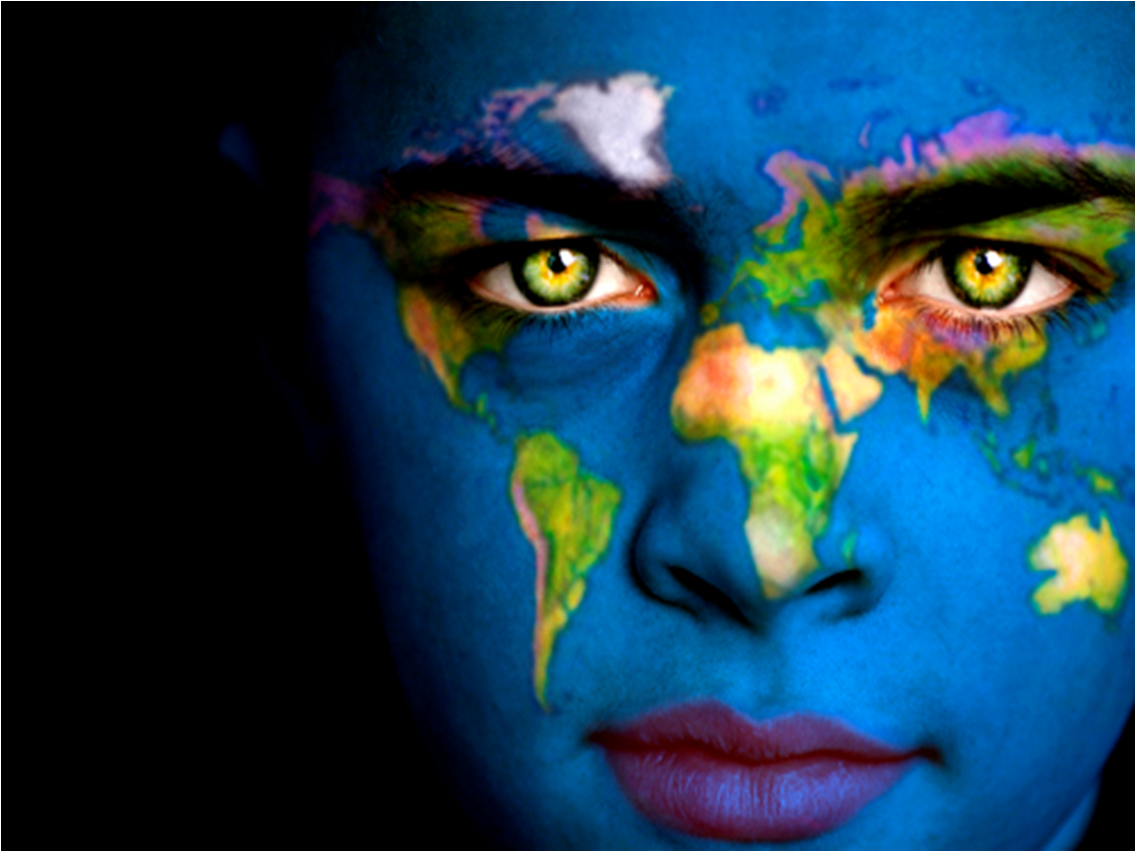
\includegraphics[height=\paperheight]{images/worldwide.png}}
\begin{frame}{Worlwide}
\end{frame}
}

\subsection{Scaling Datacenters}

\begin{frame}{Masters \& Satellites}
    \begin{columns}
        \begin{column}[c]{0.6\textwidth}
            \begin{itemize}
                \item Master Datacenters
                    \begin{itemize}
                        \item Have persistent storage
                        \item Can own GIDs
                        \item GIDs can be migrated between Master DCs
                    \end{itemize}
                \item Satellite Datacenters
                    \begin{itemize}
                        \item Don't have persistent storage
                        \item Easy to setup and decommission
                        \item Virtual/Cloud-based
                    \end{itemize}
            \end{itemize}
        \end{column}
        \begin{column}[c]{0.4\textwidth}
            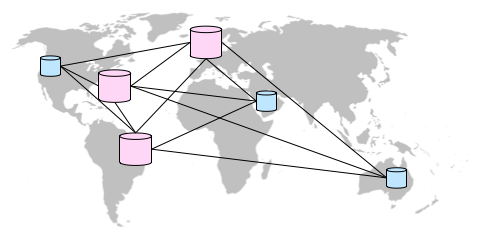
\includegraphics[width=\textwidth]{images/worldmapdc.png}
        \end{column}
    \end{columns}
\end{frame}

\begin{frame}{Start With One DC}
    \begin{center}
        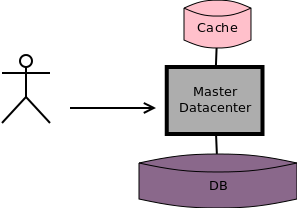
\includegraphics[width=0.4\textwidth]{images/scalingdcs1.png}
    \end{center}
\end{frame}

\begin{frame}{Scale Up A Satellite Where Needed}
    \begin{center}
        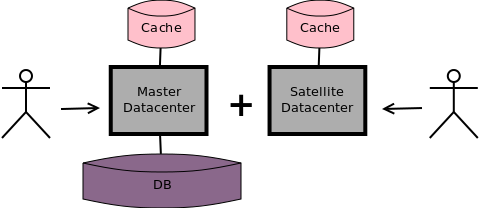
\includegraphics[width=0.7\textwidth]{images/scalingdcs2.png}
    \end{center}
\end{frame}

\begin{frame}{Turn Satellites Into Masters When Ready}
    \begin{center}
        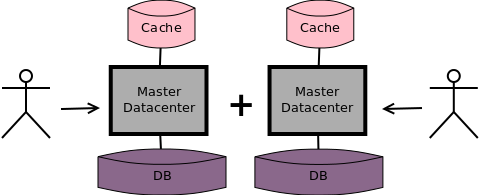
\includegraphics[width=0.7\textwidth]{images/scalingdcs3.png}
    \end{center}
\end{frame}

\begin{frame}{Working With Multiple Datacenters}
    \begin{columns}
        \begin{column}[c]{0.1\textwidth}
        \end{column}
        \begin{column}[c]{0.8\textwidth}
            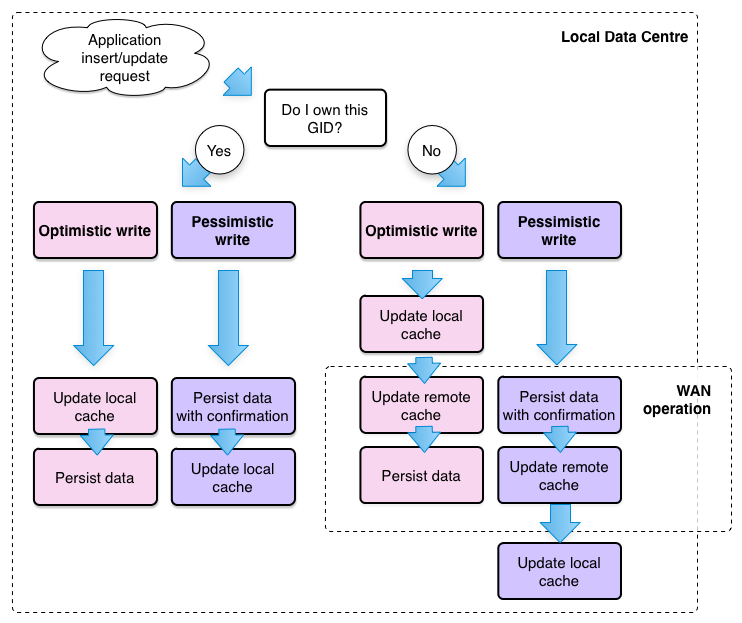
\includegraphics[width=0.8\textwidth]{images/multidcops.png}
        \end{column}
        \begin{column}[c]{0.1\textwidth}
        \end{column}
    \end{columns}
\end{frame}

\subsection{Disaster Scenarios}

{
\usebackgroundtemplate{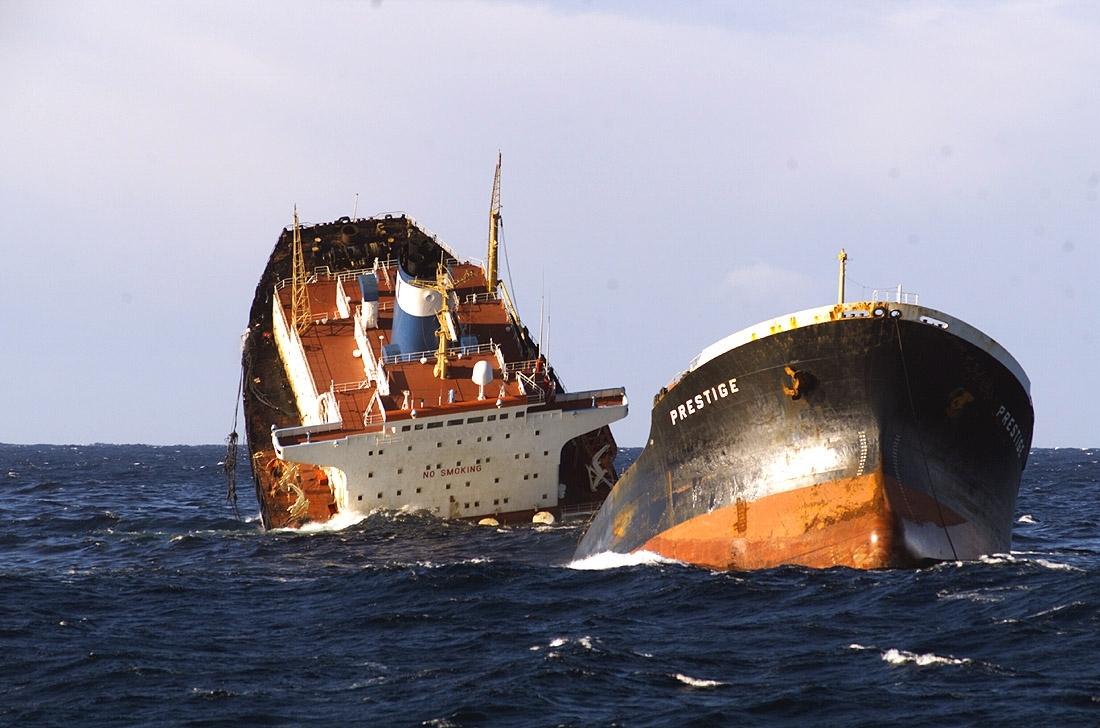
\includegraphics[height=\paperheight]{images/prestige.png}}
\begin{frame}{Disaster Scenarios}
\end{frame}
}

\begin{frame}{Losing A Satellite Datacenter}
    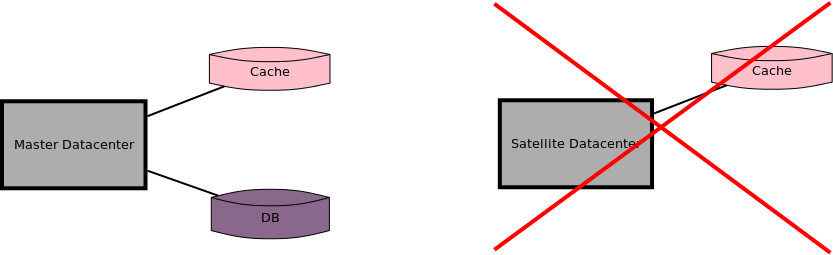
\includegraphics[width=\textwidth]{images/lostsatellitedc.png}
\end{frame}

\begin{frame}{Losing A Master Datacenter}
    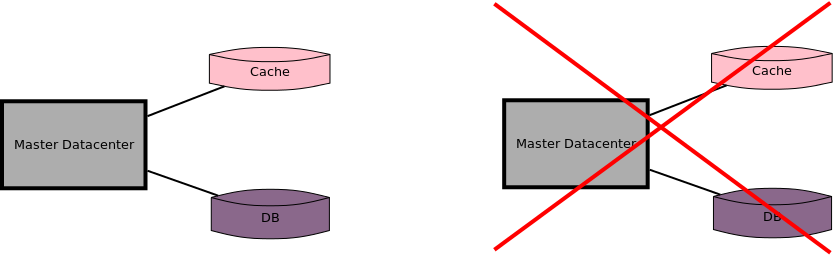
\includegraphics[width=\textwidth]{images/lostmasterdc.png}
\end{frame}

\begin{frame}{Losing A Master Datacenter}
    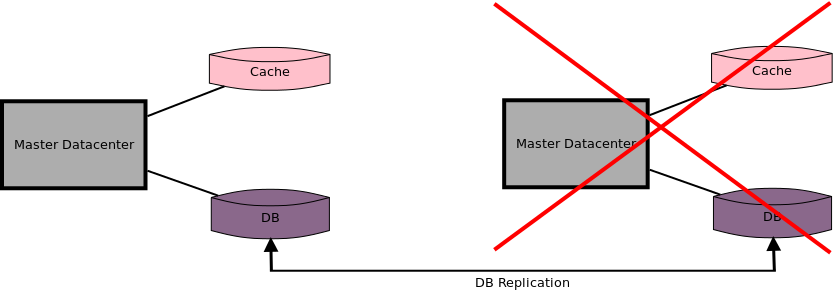
\includegraphics[width=\textwidth]{images/lostmasterdchope.png}
\end{frame}

\section{Lessons Learned}

\subsection{Currents Status}
\begin{frame}{Where We Are}
    \begin{itemize}
        \item Using simple buckets on LIVE in one DC
        \item Added relup support for bucket only updates
        \item Hammering SSP using property based testing
        \item Integrating restricted search capabilities
        \item Testing the WAN protocol for inter DC communication
        \item More buckets to go live in H1 2013
        \item Satellite DCs coming on H2 2013
    \end{itemize}
\end{frame}

\subsection{Contributions}
% TODO Links!!
\begin{frame}{What We've Used}
    \begin{itemize}
        \item \href{https://github.com/Eonblast/Emysql}{Emysql}
            \begin{itemize}
                \item
                    (\href{https://github.com/Eonblast/Emysql/commit/df25362f9cde560de680c76780d540afd43109f3}{+}) multi-database transaction support
                \item (\href{https://github.com/Eonblast/Emysql/pull/43}{*}) multi-timezone support
            \end{itemize}
        \item \href{http://github.com/davisp/eep0018}{Eep0018}/\href{http://github.com/davisp/jiffy}{Jiffy}
        \item \href{http://github.com/RJ/estatsd}{Estatsd}
        \item \href{http://github.com/manopapad/proper}{PropEr}
        \item \href{http://github.com/devinus/poolboy}{Poolboy}
        \item \href{http://github.com/basho/lager}{Lager}
        \item \href{http://github.com/basho/rebar}{Rebar}
            \begin{itemize}
                \item (\href{https://github.com/basho/rebar/pull/263}{*}) semantic versioning, i.e. [">=1.3.1", "<2.0.0"]
                \item (\href{https://github.com/basho/rebar/pull/262}{*}) shared dependencies
                \item (\href{https://github.com/rebar/rebar/pull/65}{*}) xref fixes
            \end{itemize}
        \item \href{http://github.com/alavrik/piqi}{Piqi}
        \item \href{http://github.com/basho/basho\_bench}{BashoBench}
            \begin{itemize}
                \item (\href{https://github.com/basho/basho\_bench/pull/67}{+}) Several tests on the same plot support
            \end{itemize}
    \end{itemize}
\end{frame}

\begin{frame}{Questions?}
    \begin{columns}
        \begin{column}[c]{0.5\textwidth}
            
\includegraphics[width=0.8\textwidth]{images/holycow.png}
        \end{column}
        \begin{column}[c]{0.5\textwidth}
            
\includegraphics[width=0.6\textwidth]{images/questions.png}
        \end{column}
    \end{columns}
\end{frame}

\begin{frame}{That's All Folks!}
    \begin{center}
        \huge{Thanks!}
    \end{center}
\end{frame}

\begin{frame}{Join Us!}
    \begin{center}
        
\includegraphics[width=0.5\textwidth]{images/hiring.png}\\
        \href{http://www.spilgames.com/careers/job-openings/}{\large{http://www.spilgames.com/careers/job-openings/}}
    \end{center}
\end{frame}

\end{document}

